\documentclass{article}

\usepackage{fancyhdr} % Required for custom headers
\usepackage{lastpage} % Required to determine the last page for the footer
\usepackage{extramarks} % Required for headers and footers
\usepackage[usenames,dvipsnames]{color} % Required for custom colors
\usepackage[table]{xcolor}
\usepackage{graphicx} % Required to insert images
\usepackage{listings} % Required for insertion of code
\usepackage{algpseudocode} % Required for pseudocode listing
\usepackage{courier} % Required for the courier font
\usepackage{amsmath}
\usepackage{amssymb}
\usepackage{booktabs}
\usepackage{multirow}
\usepackage{tikz}
\usetikzlibrary{arrows, shapes, positioning, calc}
\usepackage{caption}
\usepackage{wasysym}
\usepackage{multirow}
\usepackage{float}
\usepackage{tcolorbox}
\usepackage{csquotes}
\usepackage{fancybox}
\usepackage{enumitem}
\usepackage[letterspace=150]{microtype}
\usepackage{cancel}
\usepackage{hyperref}

% Margins
\topmargin=-0.45in
\evensidemargin=0in
\oddsidemargin=0in
\textwidth=6.5in
\textheight=9.0in
\headsep=0.25in

\linespread{1.1} % Line spacing

% Set up the header and footer
\pagestyle{fancy}
\lhead{\labAuthorName \; (\labAuthorUIN)} % Top left header
\chead{\labClass\  \labTitle} % Top center head
\rhead{\firstxmark} % Top right header
\lfoot{\lastxmark} % Bottom left footer
\cfoot{} % Bottom center footer
\rfoot{Page\ \thepage\ of\ \protect\pageref{LastPage}} % Bottom right footer
\renewcommand\headrulewidth{0.4pt} % Size of the header rule
\renewcommand\footrulewidth{0.4pt} % Size of the footer rule

\usepackage{fancyvrb}

\setlength\parindent{0pt} % Removes all indentation from paragraphs


%----------------------------------------------------------------------------------------
%	DOCUMENT STRUCTURE COMMANDS
%	Skip this unless you know what you're doing
%----------------------------------------------------------------------------------------

% Header and footer for when a page split occurs within a problem environment
\newcommand{\enterProblemHeader}[1]{
\nobreak\extramarks{#1}{#1 continued on next page\ldots}\nobreak
\nobreak\extramarks{#1 (continued)}{#1 continued on next page\ldots}\nobreak
}

% Header and footer for when a page split occurs between problem environments
\newcommand{\exitProblemHeader}[1]{
\nobreak\extramarks{#1 (continued)}{#1 continued on next page\ldots}\nobreak
\nobreak\extramarks{#1}{}\nobreak
}

\setcounter{secnumdepth}{0} % Removes default section numbers
\newcounter{labProblemCounter} % Creates a counter to keep track of the number of problems

\newcommand{\labProblemName}{}
\newenvironment{labProblem}[1][Problem \arabic{labProblemCounter}]{ % Makes a new environment called labProblem which takes 1 argument (custom name) but the default is "Problem #"
\stepcounter{labProblemCounter} % Increase counter for number of problems
\renewcommand{\labProblemName}{#1} % Assign \labProblemName the name of the problem
\subsection{\labProblemName} % Make a section in the document with the custom problem count
\enterProblemHeader{\labProblemName} % Header and footer within the environment
}{
\exitProblemHeader{\labProblemName} % Header and footer after the environment
}

\newcommand{\problemAnswer}[1]{ % Defines the problem answer command with the content as the only argument
\noindent\framebox[\columnwidth][c]{\begin{minipage}{0.98\columnwidth}#1\end{minipage}} % Makes the box around the problem answer and puts the content inside
}

\newcommand{\labSectionName}{}
\newenvironment{labSection}[1]{ % New environment for sections within homework problems, takes 1 argument - the name of the section
\renewcommand{\labSectionName}{#1} % Assign \homeworkSectionName to the name of the section from the environment argument
\subsection{\labSectionName} % Make a subsection with the custom name of the subsection
\enterProblemHeader{\labProblemName\ [\labSectionName]} % Header and footer within the environment
}{
\enterProblemHeader{\labProblemName} % Header and footer after the environment
}

%----------------------------------------------------------------------------------------
%	NAME AND CLASS SECTION
%----------------------------------------------------------------------------------------

\newcommand{\labTitle}{Secret Key Encryption} % Assignment title
\newcommand{\labDueDate}{10\ October,\ 2019} % Due date
\newcommand{\labClass}{CSCE\ 465} % Course/class
\newcommand{\labClassTime}{Fall 2019} % Class/lecture time
\newcommand{\labClassInstructor}{Gu} % Teacher/lecturer
\newcommand{\labAuthorName}{M. Hunter Martin} % Your name
\newcommand{\labAuthorUIN}{825002697}

%----------------------------------------------------------------------------------------
%	TITLE PAGE
%----------------------------------------------------------------------------------------

\title{
\vspace{2in}
\textmd{\textbf{\labClass\ :\ \labTitle}}\\
\normalsize\vspace{0.1in}\small{Due\ on\ \labDueDate}\\
\vspace{0.1in}\large{\textit{\labClassInstructor\ \labClassTime}}
\vspace{3in}
}

\author{\textbf{\labAuthorName}\\ \textbf{\labAuthorUIN}}
\date{}

%----------------------------------------------------------------------------------------

\begin{document}

\maketitle
\newpage

\section{Written Problems}
\begin{labProblem}[2.2 (3 pts)]
\begin{displayquote}
\begin{tcolorbox}
Random J. has been told to design a scheme to prevent messages from being modified by an intruder. Random J. decided to append to each message a hash of that message. Does this solve the problem? Why?
\end{tcolorbox}
\end{displayquote}
If we assume that an attacker can modify the message, then we know that the attacker can also modify the hash.  The attacker can simply change the message then recompute their own hash.
\end{labProblem}

\begin{labProblem}[2.3 (4 pts)]
\begin{displayquote}
\begin{tcolorbox}
Suppose Alice, Bob, and Carol want to use secret key technology to authenticate each other. If they all used the same secret key K, then Bob could impersonate Carol to Alicia (actually any of three can impersonate the other to the third). Suppose instead that each had their own secret key, so Alice uses KA, Bob uses KB, and Carol uses KC. This means that each one, to prove his/her identity, responds to a challenge with a function of his/her secret key and the challenge. Is this more secure than having them all use the same secret key K? (Hint: what does Alice need to know in order to verify Carol’s answer to Alice’s challenge?)
\end{tcolorbox}
\end{displayquote}
It is somewhat more secure, but not in a useful way.  Because these are secret keys, it is again impossible to know that the person is who they say who they are, but in theory you would be able to tell messages from Bob and Carol apart.  Essentially you know that respondent D and E are different people, but you don’t know if D is Bob or if D is Carol.
\end{labProblem}

\begin{labProblem}[2.4 (4 pts)]
\begin{displayquote}
\begin{tcolorbox}
It is common, for performance reasons, to sign a message digest of a message rather than the message itself. Why is it so important that it be difficult to find two messages with the same message digest?
\end{tcolorbox}
\end{displayquote}
If we find two messages that map to the same message digest, then we can’t verify the identity of the sender.
\end{labProblem}

\begin{labProblem}[3.2 (7 pts)]
\begin{displayquote}
\begin{tcolorbox}
Token cards display a number that changes periodically, perhaps every minute. Each such device has a unique secret key. A human can prove possession of a particular such device by entering the displayed number into a computer system. The computer system knows the secret keys of each authorized device. How would you design such a device?
\end{tcolorbox}
\end{displayquote}
The device can generate a hash between the current time and the secret key.  The user will submit the generated hash “one-time passcode,” and the computer system will recompute the hash of the time and the user’s secret key.  If the two hashes match, then the user will have verified their ownership.
\end{labProblem}

\begin{labProblem}[3.3 (7 pts)]
\begin{displayquote}
\begin{tcolorbox}
How many DES keys, on the average, encrypt a particular plaintext block to a particular ciphertext block? Please explain.
\end{tcolorbox}
\end{displayquote}
Each block of plaintext is 64 bits, and those bits are mapped to a 64 bit ciphertext output using a 56 bit key.  This means that 1 in 256 of all possible keys can map a particular plaintext block to a particular ciphertext block.
\end{labProblem}

\begin{labProblem}[3.5 (7 pts)]
\begin{displayquote}
\begin{tcolorbox}
Suppose the DES mangler function mapped every 32-bit value to zero, regardless of the value of its input. What function would DES then compute?
\end{tcolorbox}
\end{displayquote}
All DES would do is an initial permutation, the LR block swap, and the ending permutation.  The ciphertext would be a simple interchange of the odd and even bits.
\end{labProblem}

\begin{labProblem}[4.2 (7 pts)]
\begin{displayquote}
\begin{tcolorbox}
The psudo-random stream of blocks generated by 64-bit OFB must eventually repeat (since at most 264 different blocks can be generated). Will K{IV } necessarily be the first block to be repeated?
\end{tcolorbox}
\end{displayquote}
Yes.  Because we know that decryption in OFB is the inverse of encryption, we know that sequence must be repeating.
\end{labProblem}

\begin{labProblem}[4.4 (\textit{Bonus} 7 pts)]
\begin{displayquote}
\begin{tcolorbox}
What is a practical method for finding a triple of keys that maps a given plaintext to a given ciphertext using EDE? Hint: It is like the meet-in-the-middle attack mentioned in the class (detailed in the KPS textbook).
\end{tcolorbox}
\end{displayquote}
This question refers to the fact that it is relatively simple to brute force the Triple DES (3DES) encryption.  We can fix the first key, increment the second key, and increment the third key fully for each of the second key's values.  We can expect to break the 3DES algorithm relatively quickly by simply trying all of the keys.
\end{labProblem}

\begin{labProblem}[4.6 (7 pts)]
\begin{displayquote}
\begin{tcolorbox}
Consider the following alternative method of encrypting a message. To encrypt a message, use the algorithm for doing a CBC decrypt. To decrypt a message, use the algorithm for doing a CBC encrypt. Would this work? What are the security implications of this, if any, as contrasted with the “normal” CBC?
\end{tcolorbox}
\end{displayquote}
This would work, but identical plaintext blocks would produce identical ciphertext blocks.
\end{labProblem}

\section{Task 1: Encryption using different ciphers and modes [6 pts]}

I ran the following commands to encrypt the input.txt into 3 different ciphers and 3 different modes.  (AES, DES, RC2, GOST89 for the ciphers, and CBC, OFB and ECB for the modes)

\begin{verbatim}
    openssl enc -aes-128-cbc -e -in input.txt -out aes128cbc_output.bin \
    -K 00112233445566778889aabbccddeeff \
    -iv 0102030405060708
    
    openssl enc -aes-128-ofb -e -in input.txt -out aes128ofb_output.bin \
    -K 00112233445566778889aabbccddeeff \
    -iv 0102030405060708
    
    openssl enc -aes-128-ecb -e -in input.txt -out aes128ecb_output.bin \
    -K 00112233445566778889aabbccddeeff \
    -iv 0102030405060708
    
    openssl enc -des-cbc -e -in input.txt -out descbc_output.bin \
    -K 00112233445566778889aabbccddeeff \
    -iv 0102030405060708
    
    openssl enc -RC2-ECB -e -in input.txt -out rc2ecb_output.bin \
    -K 00112233445566778889aabbccddeeff \
    -iv 0102030405060708
    
    openssl enc -gost89-ecb -e -in input.txt -out gost89ecb_output.bin \
    -K 00112233445566778889aabbccddeeff \
    -iv 0102030405060708
\end{verbatim}

The input and outputs are included in Task 1 subdirectory.

\section{Task 2: Encryption Mode – ECB vs. CBC [8 pts]}
In this task I will encrypt two images using ECB and CBC.
\subsection{Trial 1: pic\_original.bmp}

This is the original picture.
\begin{center}
    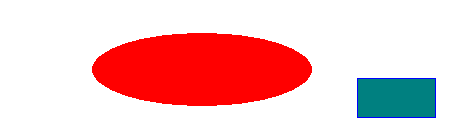
\includegraphics[scale=0.5]{pic_original.png}
\end{center}
This is encrypted using ECB.  You can notice that the shapes are still mostly visible.
\begin{center}
    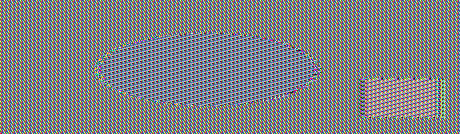
\includegraphics[scale=0.5]{pic_ecb1.png}
\end{center}
This is encrypted using CBC.  In this picture, we can't make out any of the shapes.
\begin{center}
    
\includegraphics[scale=0.5]{pic_cbc1.png}
\end{center}

\subsection{Trial 1: test2.bmp}

This is the original picture.
\begin{center}
    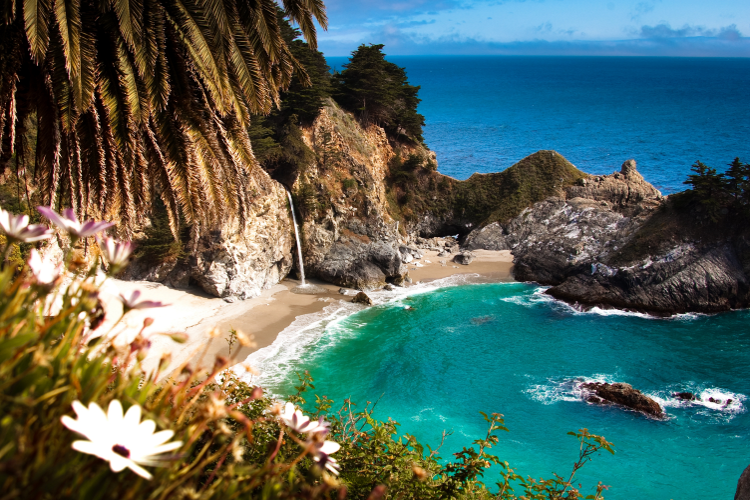
\includegraphics[scale=0.5]{test2.png}
\end{center}
This is encrypted using ECB.  You can still see the outline of a flower in the lower left hand corner.
\begin{center}
    
\includegraphics[scale=0.5]{pic_ecb2.png}
\end{center}
This is the same picture again encrypted using CBC.  In this picture, we again are unable to make out any of the shapes.
\begin{center}
    
\includegraphics[scale=0.5]{pic_cbc2.png}
\end{center}

All of the pictures are stored in the Task 2 subdirectory.

\section{Task 3: Encryption Mode – Corrupted Cipher Text [10 pts]}
Input.txt:
\begin{verbatim}
    The FitnessGram Pacer Test is a multistage aerobic capacity test that 
    progressively gets more difficult as it continues. The 20 meter pacer 
    test will begin in 30 seconds. Line up at the start. The running speed 
    starts slowly but gets faster each minute after you hear this signal 
    bodeboop. A sing lap should be completed every time you hear this sound. 
    ding Remember to run in a straight line and run as long as possible. 
    The second time you fail to complete a lap before the sound, your test is
    over. The test will begin on the word start. On your mark. Get ready, Start.
\end{verbatim}\\

In ECB, I had guessed that we'd be able to recover no data, and that was proven correct because of the dependence of the blocks.\\
\begin{center}
    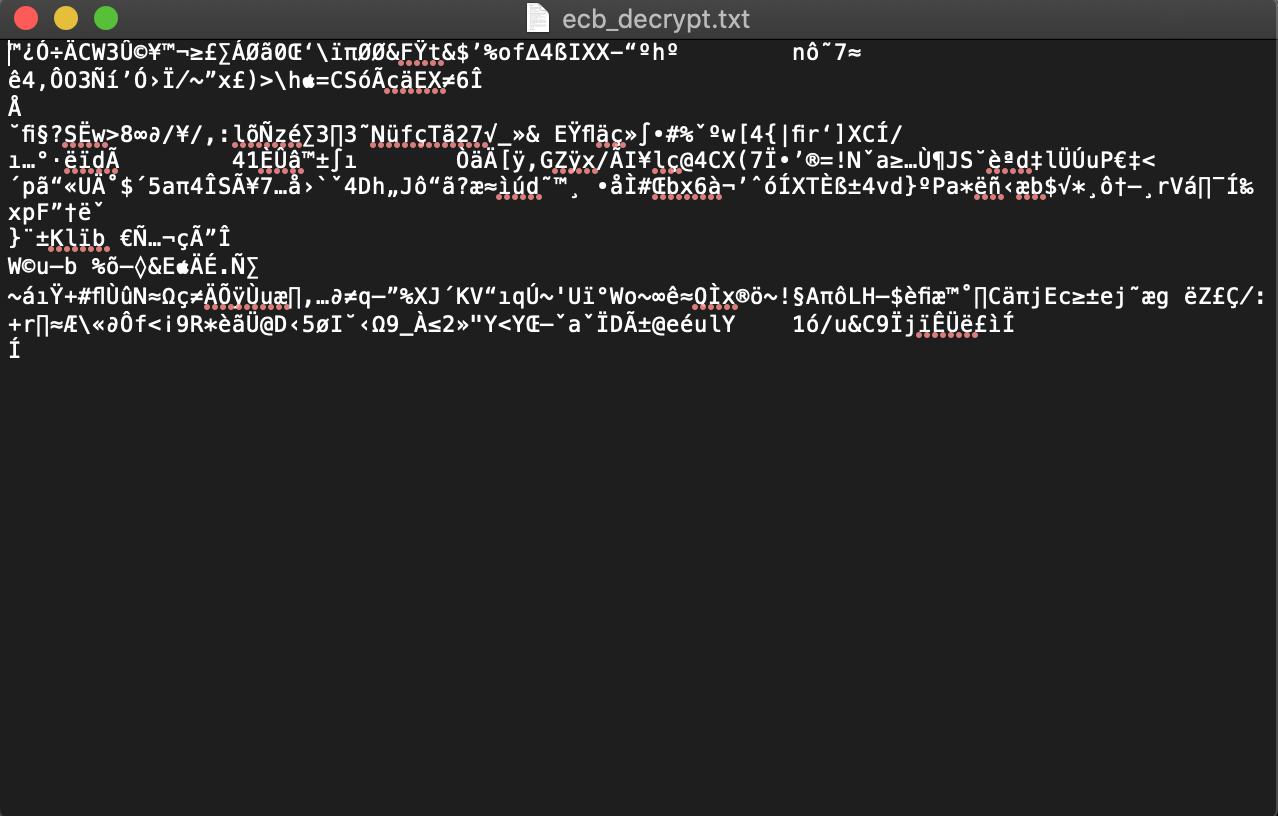
\includegraphics[scale=0.5]{ecb_decrypt.png}
\end{center}

In CBC, I had guessed that we'd be able to also recover no data, and I was again correct.  This was again because of the block dependence (errors propagate).\\
\begin{center}
    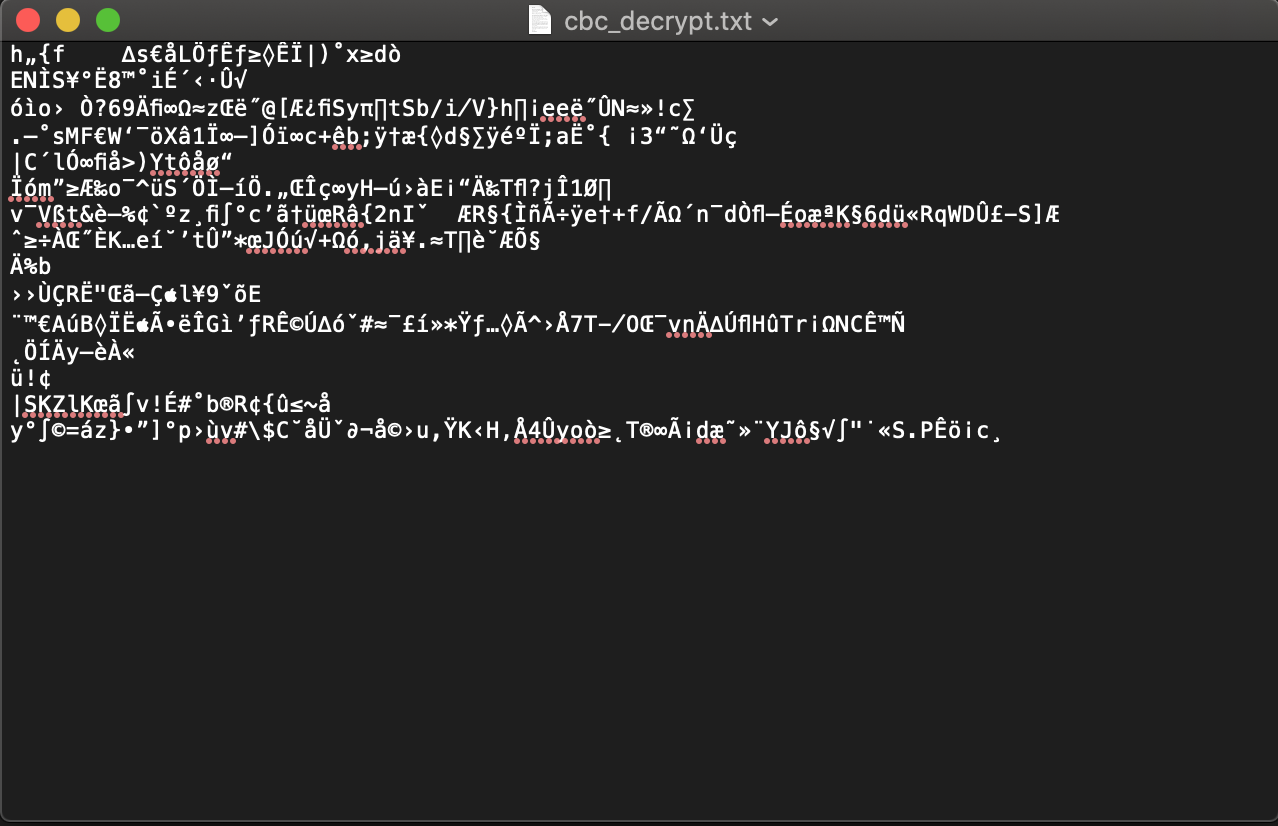
\includegraphics[scale=0.5]{cbc_decrypt.png}
\end{center}

In CFB, I had guessed that we'd be able to recover no data, but this was only partially true.  We could recover everything before the block with the error in it.  In this way, errors propagate forward but not backwards.\\
\begin{center}
    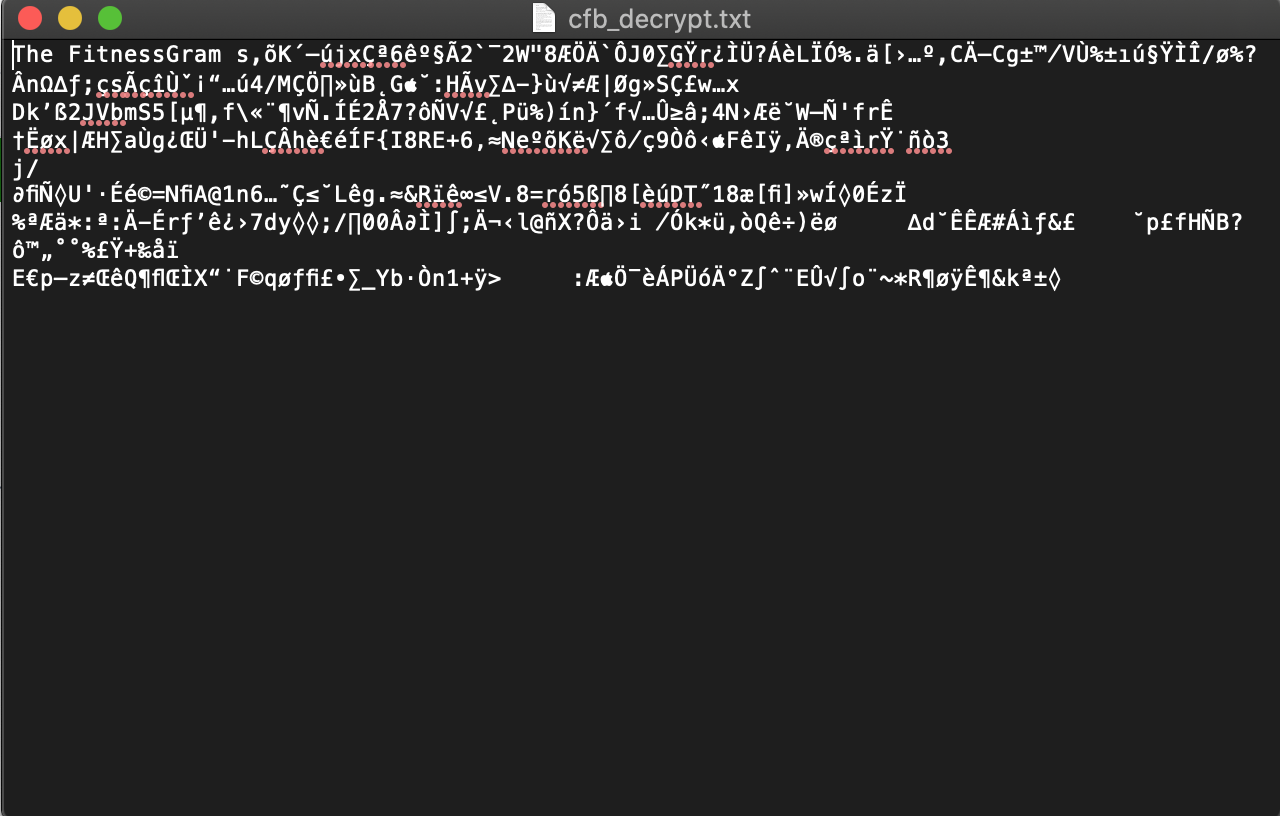
\includegraphics[scale=0.5]{cfb_decrypt.png}
\end{center}

In OFB, I had guessed that we'd be able to recover all the data not directly affected, and that was true.  Only one character was affected in the string.
\begin{verbatim}
    The FitnessGram Pacer Test is ` multistage aerobic capacity test that 
    progressively gets more difficult as it continues. The 20 meter pacer 
    test will begin in 30 seconds. Line up at the start. The running speed 
    starts slowly but gets faster each minute after you hear this signal 
    bodeboop. A sing lap should be completed every time you hear this sound. 
    ding Remember to run in a straight line and run as long as possible. 
    The second time you fail to complete a lap before the sound, your test 
    is over. The test will begin on the word start. On your mark. Get ready, Start.
\end{verbatim}\\

\section{Task 4: Programming using the Crypto Library [15 pts]}
\begin{center}
    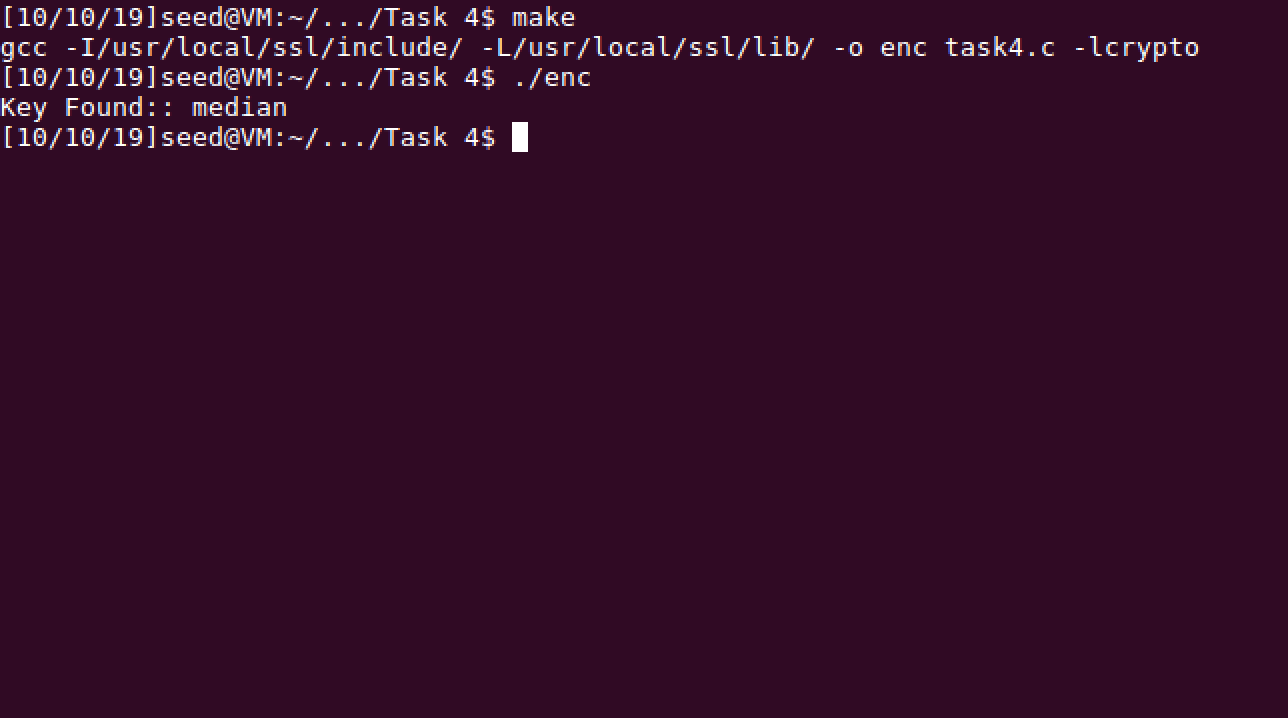
\includegraphics[scale=0.5]{task4.png}
\end{center}
Using the EVP api, I was able to determine the encryption key was "median."

\section{Task 5: Write your own DES encryption code (one round) [15 pts]}
\begin{center}
    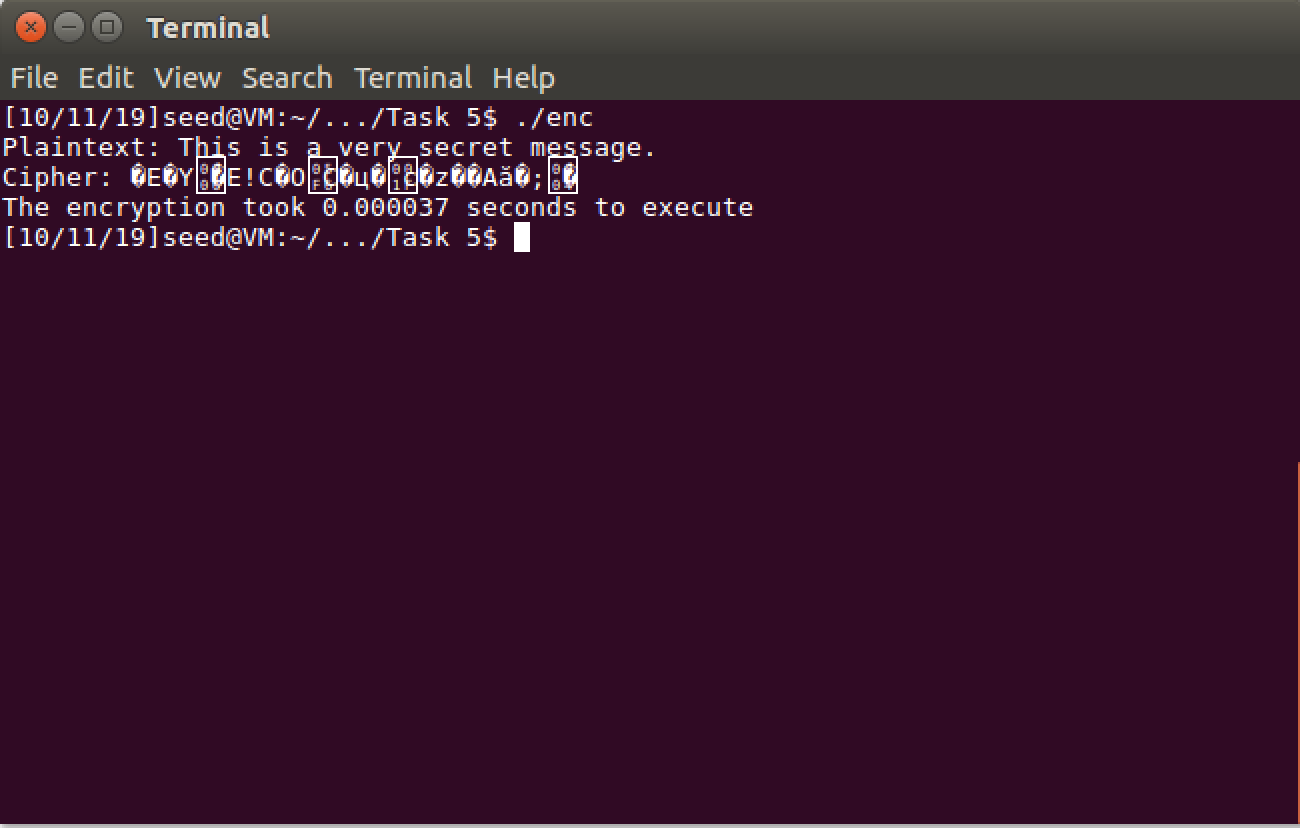
\includegraphics[scale=0.5]{task5.png}
\end{center}
My DES took on average 0.000033 seconds to complete.  I used the EVP API functions like TA Mendoza said was allowed on Oct. 6th in the comments about Task 5.

\bibliographystyle{abbrv}
\begin{thebibliography}{9}
\bibitem{assn}
Gu.
\textmd{Homework 3: Secret-Key Encryption.}
\end{thebibliography}

\end{document}